\chapter{Preliminary Validation of StARAPTOR}
\label{chap:results}

\noindent This chapter reports the preliminary validation of StARAPTOR, conducted by executing the three studies designed in Chapter~\ref{chap:methodology} (Section~\ref{sec:evaluation_methods}) on a single real-world game and reading their outcomes jointly, as prescribed by the interpretation safeguards of the methodology. The chapter follows the order of the research questions: consistency of the LLM-based extraction stage (Section~\ref{sec:rq1_results}), quality of the mined association rules (Section~\ref{sec:mining_results}), and the forecasting ablation study (Section~\ref{sec:rq3_results}) Each section is accompanied by the summarized answer to the associated research question.

\section{Study setup}
\label{sec:study_setup}

\paragraph{Case study and data.} The validation targets a single, mature, high-traffic title: Cyberpunk 2077, identified on Steam as app 1091500. The title was selected because, thanks to its constant updates, its sustained review throughput stays consistent and often exceeds the fetcher's daily ceiling of 250 reviews. Every mining window is backed by a dense set of transactions, and its player population is large and volatile, so the forecasting problem is non-trivial. The study uses one year of data: 365 daily KPI observations covering November 11, 2025 to November 11, 2026, during which the daily mean of concurrent players ranged from roughly 22{,}000 to 87{,}000, with peaks approaching 105{,}000 in the closing weeks of the observation window. Over the same period the fetcher collected 76{,}835 reviews under the stratified sampling rules described in Section~\ref{sub:data_collection} (top 125 reviews by weighted vote score plus a uniform random sample of the remainder, per day).

\paragraph{Execution environment and reproducibility.} All stages ran on a single workstation against a local, OpenAI-compatible inference endpoint (llama-cpp), with temperature 0, reasoning disabled and a concurrency limit of 8 requests, as prescribed in Section~\ref{sec:review_processing}. Every experiment was launched by a single runner script under the fixed seed 42, and the run environment (Version numbers of Python and all relevant packages, including XGBoost, Optuna, mlxtend and the Instructor-based extraction framework) was recorded in a run manifest, so that the whole study is reproducible from the recorded configuration by using the thesis branch of the project's repository\footnote{https://github.com/Mira-morphosis/StARAPTOR/tree/thesis}. The runner completed all planned studies with successful exit codes.

\paragraph{Experiment parameters.} The three studies were executed with the controlled defaults of the methodology. The RQ1 benchmark processed a frozen sample of 500 reviews drawn live from the raw, unfiltered review stream of the game (averaging over a pool of 76{,}835 raw reviews), with 1{,}000 bootstrap resamples per reliability estimate and a minimum of 30 jointly detected rating units for a stable rating-agreement estimate. The RQ2 inspection sampled rules from 52 historical mining windows (14-day windows stepped by 7 days, each containing at least 500 reviews), which stored a total of 49{,}571 mined rules. The RQ3 ablation used the chronological 70/30 split (254 training days, 110 held-out test days), 150 Optuna trials per configuration, and the recursive 30-day horizon that constitutes the system's actual deliverable.

\section{RQ1: Consistency of LLM-based Review Processing}
\label{sec:rq1_results}
\subsection{Review-level Reliability}
\noindent The benchmark compares the outputs of the four locally hosted, quantized generative models listed in Table~\ref{tab:model_configurations}, which span three performance classes by parameter count; every model processed the whole sample under identical prompts and decoding configuration, so the model is the only variable of the experiment.

\paragraph{Spam recognition.} The nominal Krippendorff's alpha over the four models' binary spam decisions is 0.797, with a 95\% bootstrap confidence interval of [0.749, 0.842]: agreement on spam recognition sits just below the 0.800 reliability threshold, i.e., at the boundary between tentative and reliable. A cross-model majority of raters flagged 114 of the 500 sampled reviews (22.8\%) as spam, confirming that the raw stream contains a substantial amount of noise that the extraction stage must absorb before the downstream stages can operate. The confidence interval does not cross the tentative threshold of 0.667, so spam recognition is at least tentatively trustworthy across models of considerably different classes.

\paragraph{Per-aspect reliability.} Table~\ref{tab:rq1_aspects} reports, for each of the 12 game aspects, the ordinal alpha computed on the full 0--5 scale consumed by the pipeline (absences included), its bootstrap confidence interval, the decomposition into detection and rating agreement, the cross-model dispersion of the daily aggregate means, and the resulting verdict according to the thresholds operationalized in Section~\ref{sub:nlp_benchmark}. Figure~\ref{fig:rq1_alpha} visualizes the same per-aspect coefficients.

\begin{longtable}{>{\columncolor{graytable}\raggedright\arraybackslash}p{0.175\linewidth} >{\centering\arraybackslash}p{0.235\linewidth} >{\centering\arraybackslash}p{0.09\linewidth} >{\centering\arraybackslash}p{0.09\linewidth} >{\centering\arraybackslash}p{0.08\linewidth} >{\centering\arraybackslash}p{0.14\linewidth}}
    \caption{Per-aspect inter-rater reliability across the four models on the frozen 500-review sample (Krippendorff's $\alpha$, ordinal variant on the full 0--5 scale, 1{,}000 bootstrap resamples). Detection and rating are the nominal (presence versus absence) and ordinal (jointly detected units only) decompositions; rating alpha is reported only when at least 30 units are jointly detected. CoV is the mean cross-model coefficient of variation of the daily aggregate feature. Verdicts follow the thresholds of Section~\ref{sub:nlp_benchmark}: reliable ($\alpha \geq 0.800$), tentative ($\alpha \geq 0.667$).}
    \label{tab:rq1_aspects}\\
    \toprule
    \rowcolor{black}
    \textbf{\textcolor{white}{Aspect}} & \textbf{\textcolor{white}{$\alpha$ ordinal [95\% CI]}} & \textbf{\textcolor{white}{Det.}} & \textbf{\textcolor{white}{Rat.}} & \textbf{\textcolor{white}{CoV}} & \textbf{\textcolor{white}{Verdict}}\\
    \bottomrule
    \endfirsthead
    \toprule
    \rowcolor{black}
    \textbf{\textcolor{white}{Aspect}} & \textbf{\textcolor{white}{$\alpha$ ordinal [95\% CI]}} & \textbf{\textcolor{white}{Det.}} & \textbf{\textcolor{white}{Rat.}} & \textbf{\textcolor{white}{CoV}} & \textbf{\textcolor{white}{Verdict}}\\
    \bottomrule
    \endhead
    \bottomrule
    \endfoot
    Multiplayer & $-0.001$ [$-0.003$, $1.000$] & $-0.001$ & n/a & 1.73 & below tentative\\
    Immersion & 0.736 [0.692, 0.784] & 0.723 & 0.728 & 0.43 & tentative\\
    Community & 0.515 [0.228, 0.691] & 0.510 & n/a & 1.10 & below tentative\\
    Replayability & 0.663 [0.610, 0.712] & 0.631 & 0.547 & 0.65 & below tentative\\
    Story & 0.870 [0.840, 0.898] & 0.872 & 0.607 & 0.20 & \textbf{reliable}\\
    Monetization & 0.416 [0.265, 0.537] & 0.420 & n/a & 1.19 & below tentative\\
    Gameplay & 0.656 [0.609, 0.703] & 0.658 & 0.722 & 0.43 & below tentative\\
    Controls & 0.412 [0.217, 0.599] & 0.410 & n/a & 1.18 & below tentative\\
    Graphics & 0.796 [0.748, 0.839] & 0.777 & 0.598 & 0.49 & tentative\\
    Customization & 0.684 [0.603, 0.755] & 0.679 & n/a & 0.78 & tentative\\
    Audio & 0.892 [0.844, 0.933] & 0.885 & 0.763 & 0.28 & \textbf{reliable}\\
    Difficulty & 0.731 [0.592, 0.840] & 0.730 & n/a & 0.80 & tentative\\
\end{longtable}


\begin{figure}[H]
    \centering
    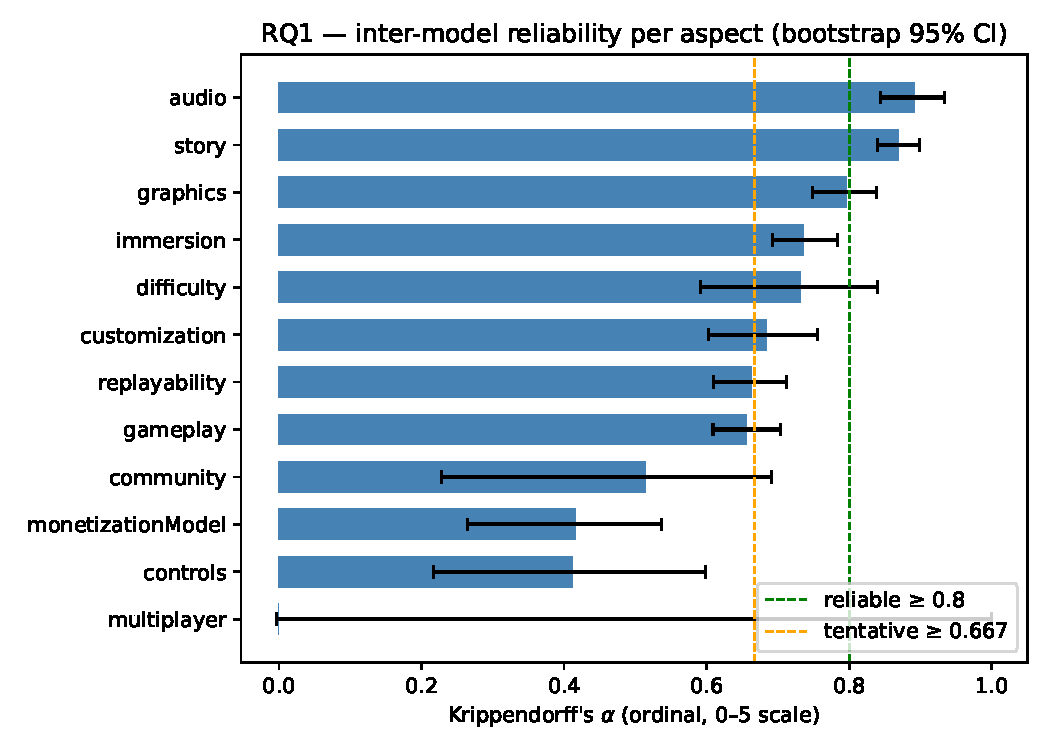
\includegraphics[width=0.9\linewidth]{figure/results_rq1_alpha_per_aspect.pdf}
    \caption{Per-aspect inter-rater reliability of the extraction stage across the four benchmarked models (Krippendorff's $\alpha$). Error bars show the 95\% bootstrap confidence intervals; the vertical lines mark the reliability (0.800) and tentative (0.667) thresholds used to grade the verdicts.}
    \label{fig:rq1_alpha}
\end{figure}

The picture that emerges is strongly aspect-dependent, which is itself the most informative outcome of the benchmark. Agreement is \textbf{reliable} for exactly two aspects, audio (0.892) and story (0.870): these are the aspects the models both detect consistently and score coherently, and for them the confidence intervals lie entirely above the 0.800 threshold. Four aspects are \textbf{tentative}: graphics (0.796, whose upper confidence bound reaches 0.839), immersion (0.736), difficulty (0.731) and customization (0.684). Gameplay (0.656) and replayability (0.663) fall just below the tentative threshold, although their intervals nearly touch 0.667 and their rating-agreement components (0.722 and 0.547 respectively) confirm that at least the core gameplay judgment is coherently scored when detected. Community (0.515), monetization (0.416) and controls (0.412) show weak agreement, and multiplayer is at chance level: being it an absent feature in the examined videogame, this is expected behaviour; however, this finding makes clear that results to the first Research Question are possibly game dependent, so this has to be considered a limitation of the study.

Two regularities qualify the numbers. First, the detection and rating components diverge in an instructive way: for gameplay the rating agreement (0.722) exceeds the detection agreement (0.658), and for audio the two components are close (0.885 and 0.763), indicating that once models agree that an aspect is discussed, they tend to agree on the score as well. The residual unreliability is concentrated in the detection decision, i.e., in whether an aspect is explicitly discussed at all, which is the harder semantic judgment for borderline mentions. Second, the aspects that fail are exactly those that are structurally hard to separate: monetization overlaps with general complaints about value, controls overlap with bug reports, community and multiplayer complaints are often not discussed explicitly (as also found by Li et al. \cite{ethical_game_dev_reddit})

\subsection{Aggregate-level Dispersion} \noindent The system also consumes the processed reviews in aggregated windows, so a benchmark measures the dispersion of the daily aggregate features that feed the forecasting stage. Over the 248 days with valid aggregates across all models, the mean cross-model coefficient of variation of the daily mean score is 0.20 for story and 0.28 for audio, matching their reliable per-review alphas; it stays below 0.50 for immersion, gameplay and graphics; and it exceeds 1.0 for community, controls, monetization and multiplayer. The daily positive-review ratio, the single most review-dependent scalar feature of the forecasting matrix, is highly stable across models, with a coefficient of variation of 0.06. The ordering of aggregate dispersion therefore tracks the ordering of per-aspect reliability: the features the pipeline consumes most densely are precisely the ones the models agree on, and averaging by day suppresses much of the per-review disagreement, as the aggregation of many noisy but roughly independent judgments is expected to do.

\rqanswer{1}{Yes. Its consistency is acceptable, but possibly game-dependent. Models with higher parameter counts tend to be more consistent than smaller ones; the two largest models (\texttt{Qwen3.8-27B} and \texttt{Muse-Glimmer-30B}) have the highest agreement rate and the smallest agreement rate delta, with the gap widening across size classes, so the system benefits from the use of large language models.}

\subsection{Model choice for next experiments} \noindent Under the consensus criterion of Section~\ref{sub:nlp_benchmark}, the base model was selected by the highest cross-model majority agreement. The selected model was \texttt{Qwen3.8-27B} (Agreement rate: 0.908), which then re-processed the entire fetched review pool of 76{,}835 reviews with zero extraction failures, persisting 76{,}415 new extractions and refreshing the 420 overlapping ones, so that RQ2 and RQ3 operate on a single consistent labeling of the whole history.

\section{RQ2: Quality of the Mined Association Rules}
\label{sec:mining_results}

\noindent The inspection study applies the fixed, pre-registered protocol of Section~\ref{subsec:rules_verification} to the rules mined over the game's history. Sampling drew, for each of the 52 historical mining windows, the top 10 rules by lift plus 5 uniformly random rules from the remainder, using the fixed seed 42, yielding 765 distinct sampled rules; the same seed governs all random components of the study, so the sample is exactly reproducible. Every rule was classified by the deterministic decision procedure of Table~\ref{tab:classification_rules}, and every rule classified as actionable was traced back to its supporting reviews (up to 10 per rule), all of which were retrieved from the study database, providing the grounding evidence the protocol requires.

\paragraph{Category distribution and residual noise.} Table~\ref{tab:rq2_categories} reports the outcome of the classification. Of the 765 inspected rules, 564 (73.7\%) are actionable, i.e., they connect semantic review content, such as aspect scores, bug-related flags and playtime buckets, to semantically rich patterns a developer could act upon. The residual noise rate, i.e., the fraction of sampled rules that the filter cascade should have removed (semantically trivial plus taxonomy artifacts, excluding the unclear ones), is 18.8\%. Its composition is informative: taxonomy artifacts, the rules whose association is mediated by the item structure rather than by the domain (language, hardware, purchase attributes), are almost eliminated by the cascade (11 rules, 1.4\%), and the bulk of the residual is semantically trivial rules (133, 17.4\%), mostly restatements of the overall review polarity via the entailment relations between the extracted flags. The unclear category, associations near statistical independence, accounts for the remaining 7.5\%.

\begin{table}[H]
    \centering
    \caption{Distribution of the 765 sampled mined rules across the four categories of the pre-registered inspection rubric, together with the derived quality metrics. The decision procedure and the thresholds are those of Table~\ref{tab:classification_rules}.}
    \label{tab:rq2_categories}
    \begin{tabular}{lrrp{0.5\linewidth}}
        \toprule
        \rowcolor{black}
        \textbf{\textcolor{white}{Category}} & \textbf{\textcolor{white}{Rules}} & \textbf{\textcolor{white}{Share}} & \textbf{\textcolor{white}{Reading}}\\
        \midrule
        Actionable & 564 & 73.7\% & grounded and interpretable as developer insight\\
        Semantically trivial & 133 & 17.4\% & restates polarity or flag definitions\\
        Taxonomy artifact & 11 & 1.4\% & mediated by structural items\\
        Unclear & 57 & 7.5\% & near statistical independence\\
        \midrule
        Residual noise rate & 144 & 18.8\% & trivial plus artifacts\\
        Actionability rate & 564 & 73.7\% & actionable over all inspected\\
        \bottomrule
    \end{tabular}
\end{table}

\paragraph{Cross-window persistence and redundancy.} Of the 49{,}571 rules mined over the 52 windows, 8{,}861 (17.9\%) recur in more than one independent window, indicating that a substantial minority of the discovered associations are stable properties of the game's feedback rather than artifacts of a single period. Within the inspected sample, persistence is lower (80 rules, 10.5\%), which is consistent with the sample's composition: prominence rules are selected precisely because they are extreme in their window, and extreme associations tend to be period-specific. Redundancy is the weakest point of the current cascade: 281 of the 765 sampled rules (36.7\%) share their full item-set signature with another sampled rule, and 60.0\% share their antecedent with at least one other sampled rule, i.e., multiple surviving rules describe the same underlying pattern from slightly different angles. The sub/super-redundancy pruning of Section~\ref{sec:mining_pipeline} removes strict specializations, but near-duplicate permutations resurface across windows because each window is mined independently.

\paragraph{Conclusions.} The filter cascade is largely adequate at its stated goal: the statistically valid but semantically empty patterns that motivate it, in particular fully structural hardware rules, are almost completely gone, and the actionability rate of almost three quarters certifies that the surfaced rules are predominantly interpretable as developer-facing insight. The residual noise is concentrated in a single, well-identified failure mode, polarity restatement through label entailment, which a targeted extension of the entailment filter (e.g., extending R2 of the decision procedure to the miner itself) could address. Finally, the redundancy figures show that the rule set, while informative, is still far more verbose than its information content requires, which motivates strengthening the cross-window de-duplication of the persistence stage.

\rqanswer{2}{Yes. 73.7\% of surfaced rules are actionable, i.e., grounded in review content and interpretable as developer insight. Taxonomy artifacts are nearly eliminated (1.4\% residual), but residual noise (18.8\%, dominated by polarity restatement) and redundancy (36.7\% duplicated signatures) show the rule set is noisier and more verbose than it needs to be. Alternative solutions will be explored in Chapter~\ref{chap:conclusions}.}

\section{RQ3: Forecasting Ablation}
\label{sec:rq3_results}

\noindent The ablation trains the forecasting pipeline three times on the same chronological split, holding everything constant except the feature set: C1 (baseline, 13 features, replicating a KPI-only forecaster), C2 (27 features, adding the daily review aggregates) and C3 (full system, 31{,}561 features, adding one lift feature per mined association rule). Each configuration received its own Optuna tuning pass of 150 trials, and evaluation covers both the one-day-ahead prediction and the recursive 30-day forecast on the 110 held-out test days. Figure~\ref{fig:rq3_forecast} shows the full-system forecast against the actual series over the evaluation horizon.

\begin{table}[H]
    \centering
    \caption{Forecasting metrics of the ablation configurations on the held-out test period (110 days). One-day and 30-day errors are reported as MAPE; the 30-day MAE is in mean concurrent players. Weekday and weekend columns decompose the 30-day MAPE; the underestimation rate is the fraction of forecast days below the actual value.}
    \label{tab:rq3_metrics}
    \small
    \begin{tabular}{lrrrrrrr}
        \toprule
        \rowcolor{black}
        \textbf{\textcolor{white}{Config}} & \textbf{\textcolor{white}{Features}} & \textbf{\textcolor{white}{1-day}} & \textbf{\textcolor{white}{MAE$_{30}$}} & \textbf{\textcolor{white}{MAPE$_{30}$}} & \textbf{\textcolor{white}{Weekday}} & \textbf{\textcolor{white}{Weekend}} & \textbf{\textcolor{white}{Under.}}\\
        \midrule
        C1 (baseline) & 13 & 2.55\% & 4{,}829 & 10.15\% & 9.60\% & 11.67\% & 5.83\%\\
        C2 (+ reviews) & 27 & 2.55\% & 7{,}165 & 14.59\% & 14.77\% & 14.09\% & 13.02\%\\
        C3 (+ rules) & 31{,}561 & 2.88\% & 6{,}790 & 15.40\% & 13.83\% & 19.72\% & 1.77\%\\
        \bottomrule
    \end{tabular}
\end{table}

\paragraph{Primary outcome.} The monotonic improvement from C1 to C2 to C3 that would answer RQ3 positively does not materialize on this game. One-day-ahead accuracy is essentially flat across configurations (MAPE between 2.55\% and 2.88\%, with C2 marginally better than the baseline in absolute error), because at the one-day horizon the KPI lags dominate all feature sets. The differences appear on the recursive 30-day horizon, and they run against the full system: C1 achieves the best 30-day MAPE (10.15\%), C2 degrades it by 43.7\% in relative terms (14.59\%), and C3 degrades it by 51.7\% (15.40\%). The held-out period contains a pronounced late-2026 growth episode with peaks beyond almost all training levels, a regime favorable to the smoother KPI-only baseline and hostile to any additional feature that injects variance into the recursive chain.

\paragraph{Possible causes for performance degradation.} The decomposition by day type shows that the C2 degradation is uniform across weekdays (14.77\% versus 9.60\% for the baseline), while the additional step from C2 to C3 concentrates almost entirely on weekends, where C3 reaches 19.72\%. Weekend days are exactly where the review-derived features are sparsest (fewer reviews are published, so daily aggregates and rule lifts are computed from smaller samples), so the added features carry the least information precisely where they hurt the most. The regression tree can split on them regardless, and in the recursive setting every noisy split compounds over the 30 chained predictions.

\paragraph{Underestimation and feature importance.} The one capacity-oriented metric moves in the opposite direction: the underestimation rate, which the asymmetric objective is designed to suppress, improves from 5.83\% (C1) to 13.02\% (C2) and then to 1.77\% (C3), a 69.6\% relative reduction of C1's underestimation, and 1.41\% on weekend days. The full system is thus the configuration least likely to under-provision, at the cost of raw accuracy. The gain-based importance of the C3 model shows that the regressor does rely on the mined associations: rule features absorb 52.3\% of the total split gain. The reliance, however, is extremely diffuse (the single highest-gain rule accounts for only 3.4\% of the total gain), in a feature space of 31{,}561 candidate features trained on 254 samples, a ratio of over 120 features per training point that invites variance absorption. Consistently with the interpretation safeguards of Section~\ref{sub:forecasting_evaluation}, the highest-gain rules must be read jointly with the RQ2 study: the top rule links English-language non-recommending reviews to explicit negative aspects, the second links mid-range story scores to reviews mixing positive and negative aspects, and the ninth is a purely structural hardware pattern (32 GB RAM and 16 GB VRAM machines associated with Windows 11 and Steam purchases) that the RQ2 rubric classifies as a taxonomy artifact. The regressor, in other words, does not only exploit the actionable signal that RQ2 certifies; it also absorbs structured noise that the mining cascade filters for display but that the forecasting matrix still contains.

\begin{figure}[H]
    \centering
    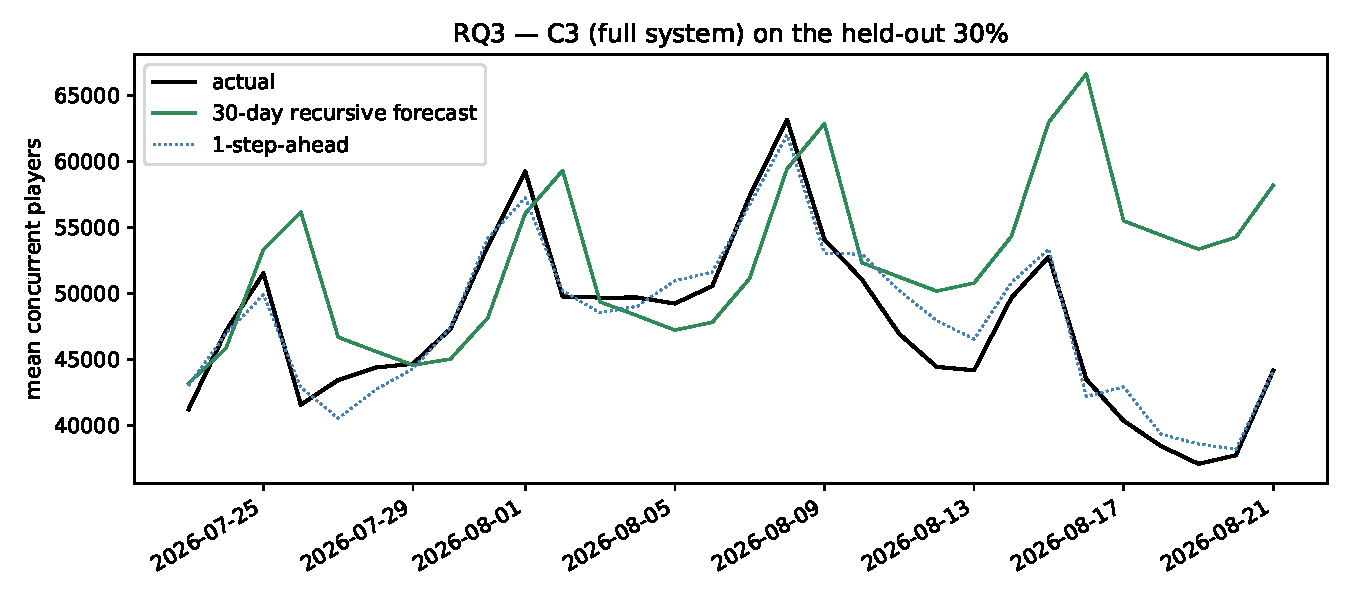
\includegraphics[width=0.9\linewidth]{figure/results_rq3_forecast_vs_actual_C3.pdf}
    \caption{Recursive 30-day forecast of the full system (C3) against the actual daily mean concurrent players over the held-out test period. The evaluation window includes the late-2026 growth episode, with player levels exceeding those observed at training time.}
    \label{fig:rq3_forecast}
\end{figure}

\begin{figure}[H]
    \centering
    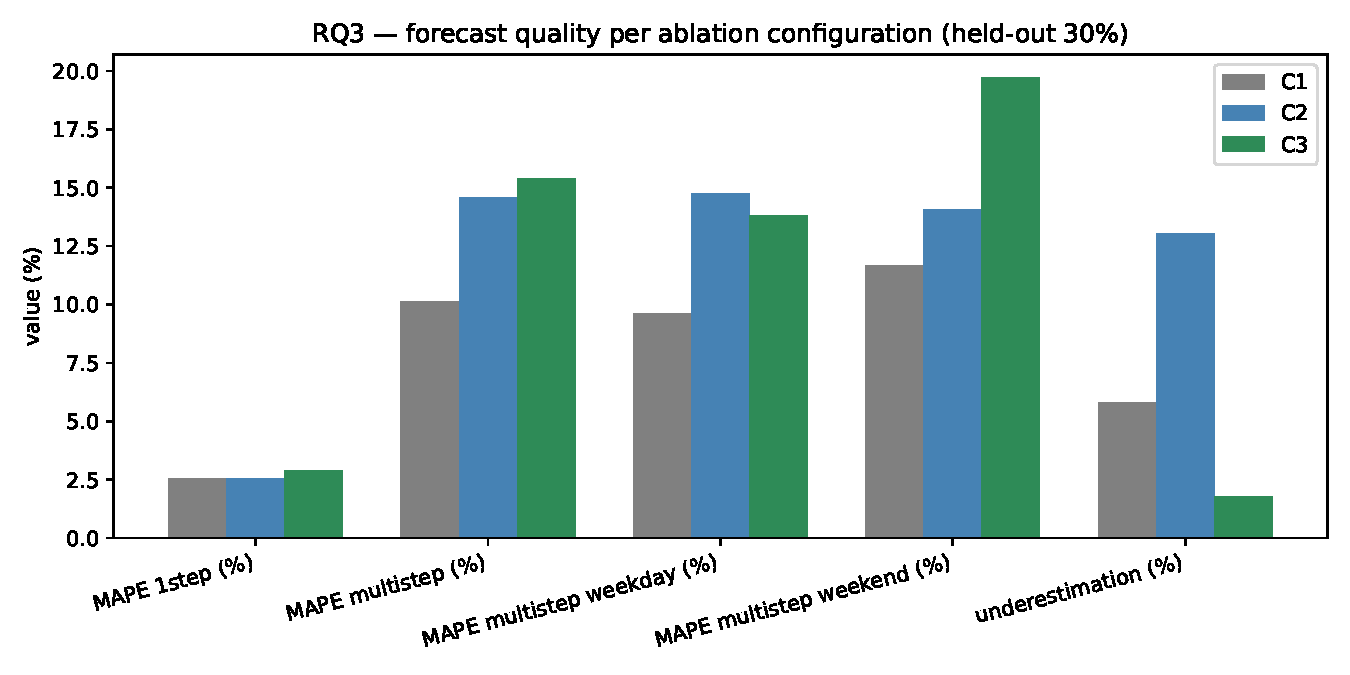
\includegraphics[width=0.9\linewidth]{figure/results_rq3_metrics_by_config.pdf}
    \caption{Forecasting error metrics by ablation configuration. One-day-ahead errors are comparable across configurations; the differences concentrate on the recursive 30-day horizon, where the KPI-only baseline (C1) remains the most accurate.}
    \label{fig:rq3_metrics}
\end{figure}

\rqanswer{3}{Not on this game, and possibly game and review dependent. The ablation shows monotonic performance degradation on the 30 days recursive forecast: review aggregates and rule features do not change one-day accuracy and degrade the recursive 30-day MAPE by 43.7\% and 51.7\% respectively against the internal KPI-only baseline. 
A partially positive result is that C3 reduces the baseline’s underestimation rate by 69.6\% in relative terms. As the study is
preliminary and single-game, RQ3 must be read as open rather than settled, with the evidence identifying the candidate causes to address: variance injection into the recursive chain, sparse rule features relative to the training size, and structural rules surviving in the feature matrix as the highest gain rules. This experiment's conclusions will be expanded in Chapter~\ref{chap:conclusions}.}